

\subsection{Áttekintés}

\subsubsection{Általános áttekintés}

\begin{figure}[ht!]
	\centering
	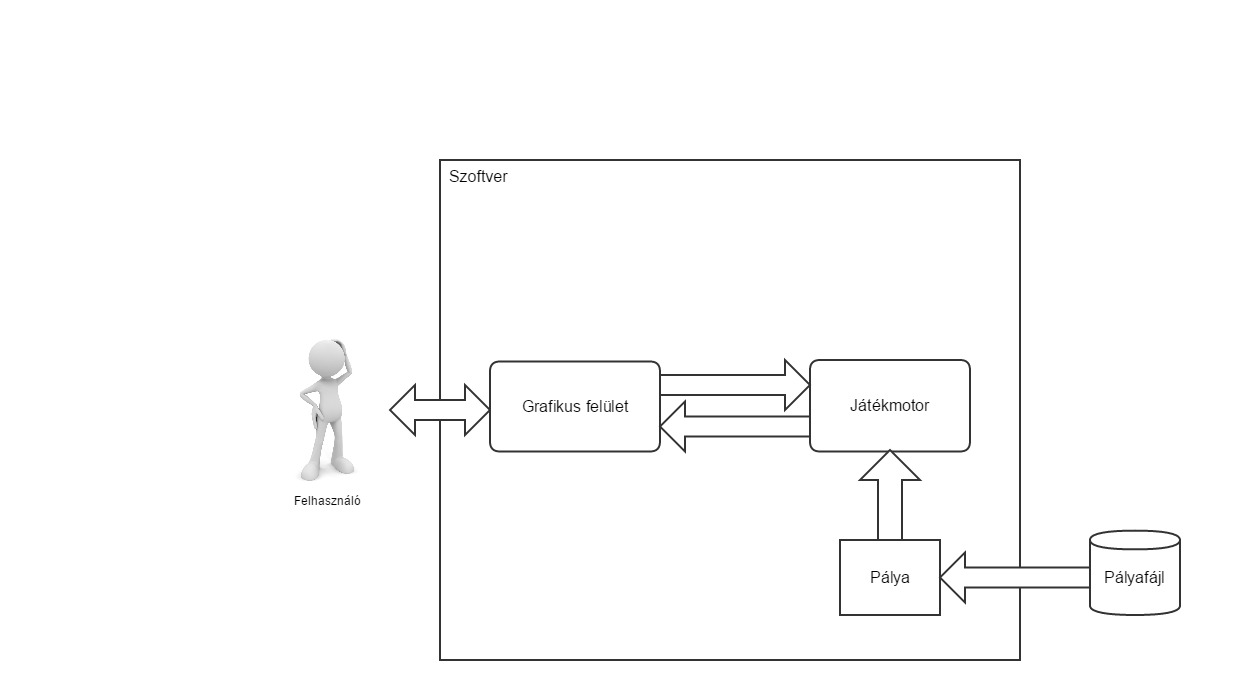
\includegraphics[width=180mm, center]{./chapters/chapter02/dia1.jpg}
	\caption{Architekturális kép \label{overflow}}
\end{figure}

A szoftverünk legfontosabb komponense a játékmotor. Itt zajlanak le a számítások, ez futtatja a logikát, ami érzékeli, hogy egy robot elhagyta a pályát, esetleg beleugrott egy ragacsba, vagy egy olajfoltba. A játékmotor feladata az is, hogy észrevegye, amikor vége van a játéknak, azaz lejárt az idő, vagy csak egy robot maradt a pályán. \\

A grafikus felület a felhasználó számára megjeleníti a játékot, valamint ezen keresztül tudja befolyásolni a játékmotorban történő eseményeket. \\

Az előre elkészített pályát egy külső fájlból érjük el, ezt tartja nyilván a Pálya modul. A játékmotor természetesen hozzáfér ehhez, hiszen neki kell eldöntenie a robotok kezdőpozícióját, valamint az előre legenerált ragacsok és olajfoltok elhelyezkedését. \\

\subsubsection{Funkciók}

A szoftverünk ugráló robotok versenyzését szimuláló játék. Először álló helyzetből indulnak, mindegyik egy előre generált pozícióból. Mindegyik robot sebessége ugyanakkora (nevezzük egységnyi méretűnek), ami azonban tetszőleges irányú sebességvektorral változtatható. A robotok mozgása kvantált, ugrásokra bontható. Minden egyes ilyen ugrás hossza a sebességgel egyenesen arányos. \\

A játékot különlegessé tevő funkciók a pályán lévő, a robotok sebességét befolyásoló foltokhoz kapcsolódnak:

\begin{itemize}
	\item Az egyik ilyen az olajfolt, amelynek hatására a robot sebessége nem módosítható, azaz a következő ugrás sebességvektora meg fog egyezni az előző ugráséval, ami a pályaelhagyáshoz vezethet, ami a robot számára a játék végét jelenti.
	\item A másik lehetséges folt a ragacs. Ez minden esetben megfelezi a robot sebességét, tehát lassító hatással bír. Az idő lejártához közeledve nyilvánvaló, hogy a ragacsba való belépés akár az első hely elvesztésével is járhat, ezért célszerű elkerülni.
\end{itemize}

Külön érdekes az, hogy a robot a felhasználó utasítására képes az ugrása előtt maga mögött hagyni egy tetszőleges foltot. Ezen funkció hatékony használata jelentősen hozzásegítheti az adott robotot a győzelem. \\

Az a robot nyer, aki a játékidő lejárása pillanatában a legtöbb távolságot tette meg.
 

\subsubsection{Felhasználók}

A szoftver egy felhasználóra van tervezve, aki számára a játék könnyedén elsajátítható, amennyiben ismeri a szótárban megnevezett definíciókat.

\subsubsection{Korlátozások}

Korlátozásként megfogalmazható az, hogy a forrásprogramnak a laboratóriumban rendszeresített JDK alatt lefordíthatónak és futtathatónak kell lennie, nem adható hozzá külső package.

\subsubsection{Feltételezések, kapcsolatok}

Szoftver labor 4 feladatkiírás: \textit{https://www.iit.bme.hu/$\sim$szoftlab4/feladat.shtml}